\section{Results}

\subsection{Preprocessing Performance}


\subsection{OCR Evaluation}
\subsubsection{PP-OCRv4}
The performance of the text detection model is evaluated using Precision, Recall, and F1-score, based on the Intersection over Union (IoU) between predicted bounding boxes and ground truth annotations with an IoU threshold of 0.5.

\begin{table}[H]
  \centering
  \label{tab:detection_metrics}
  \begin{tabular}{lccc}
    \toprule
    \textbf{Metrics} & Precision & Recall & F1-score \\
    \midrule
    \textbf{Value}   & 0.9383    & 0.8951 & 0.9162   \\
    \bottomrule
  \end{tabular}
  \caption{Detection Performance Metrics}
\end{table}

\noindent The model achieves a precision of 93.83\%, a recall of 89.51\%, and an F1-score of 91.62\%, obtained from 17,313 true positives, 1,139 false positives, and 2,029 false negatives. The high precision indicates that most predicted text regions correspond to actual text instances, while the recall demonstrates that the model successfully detects the majority of text regions in the dataset.

\begin{figure}[H]
  \centering
  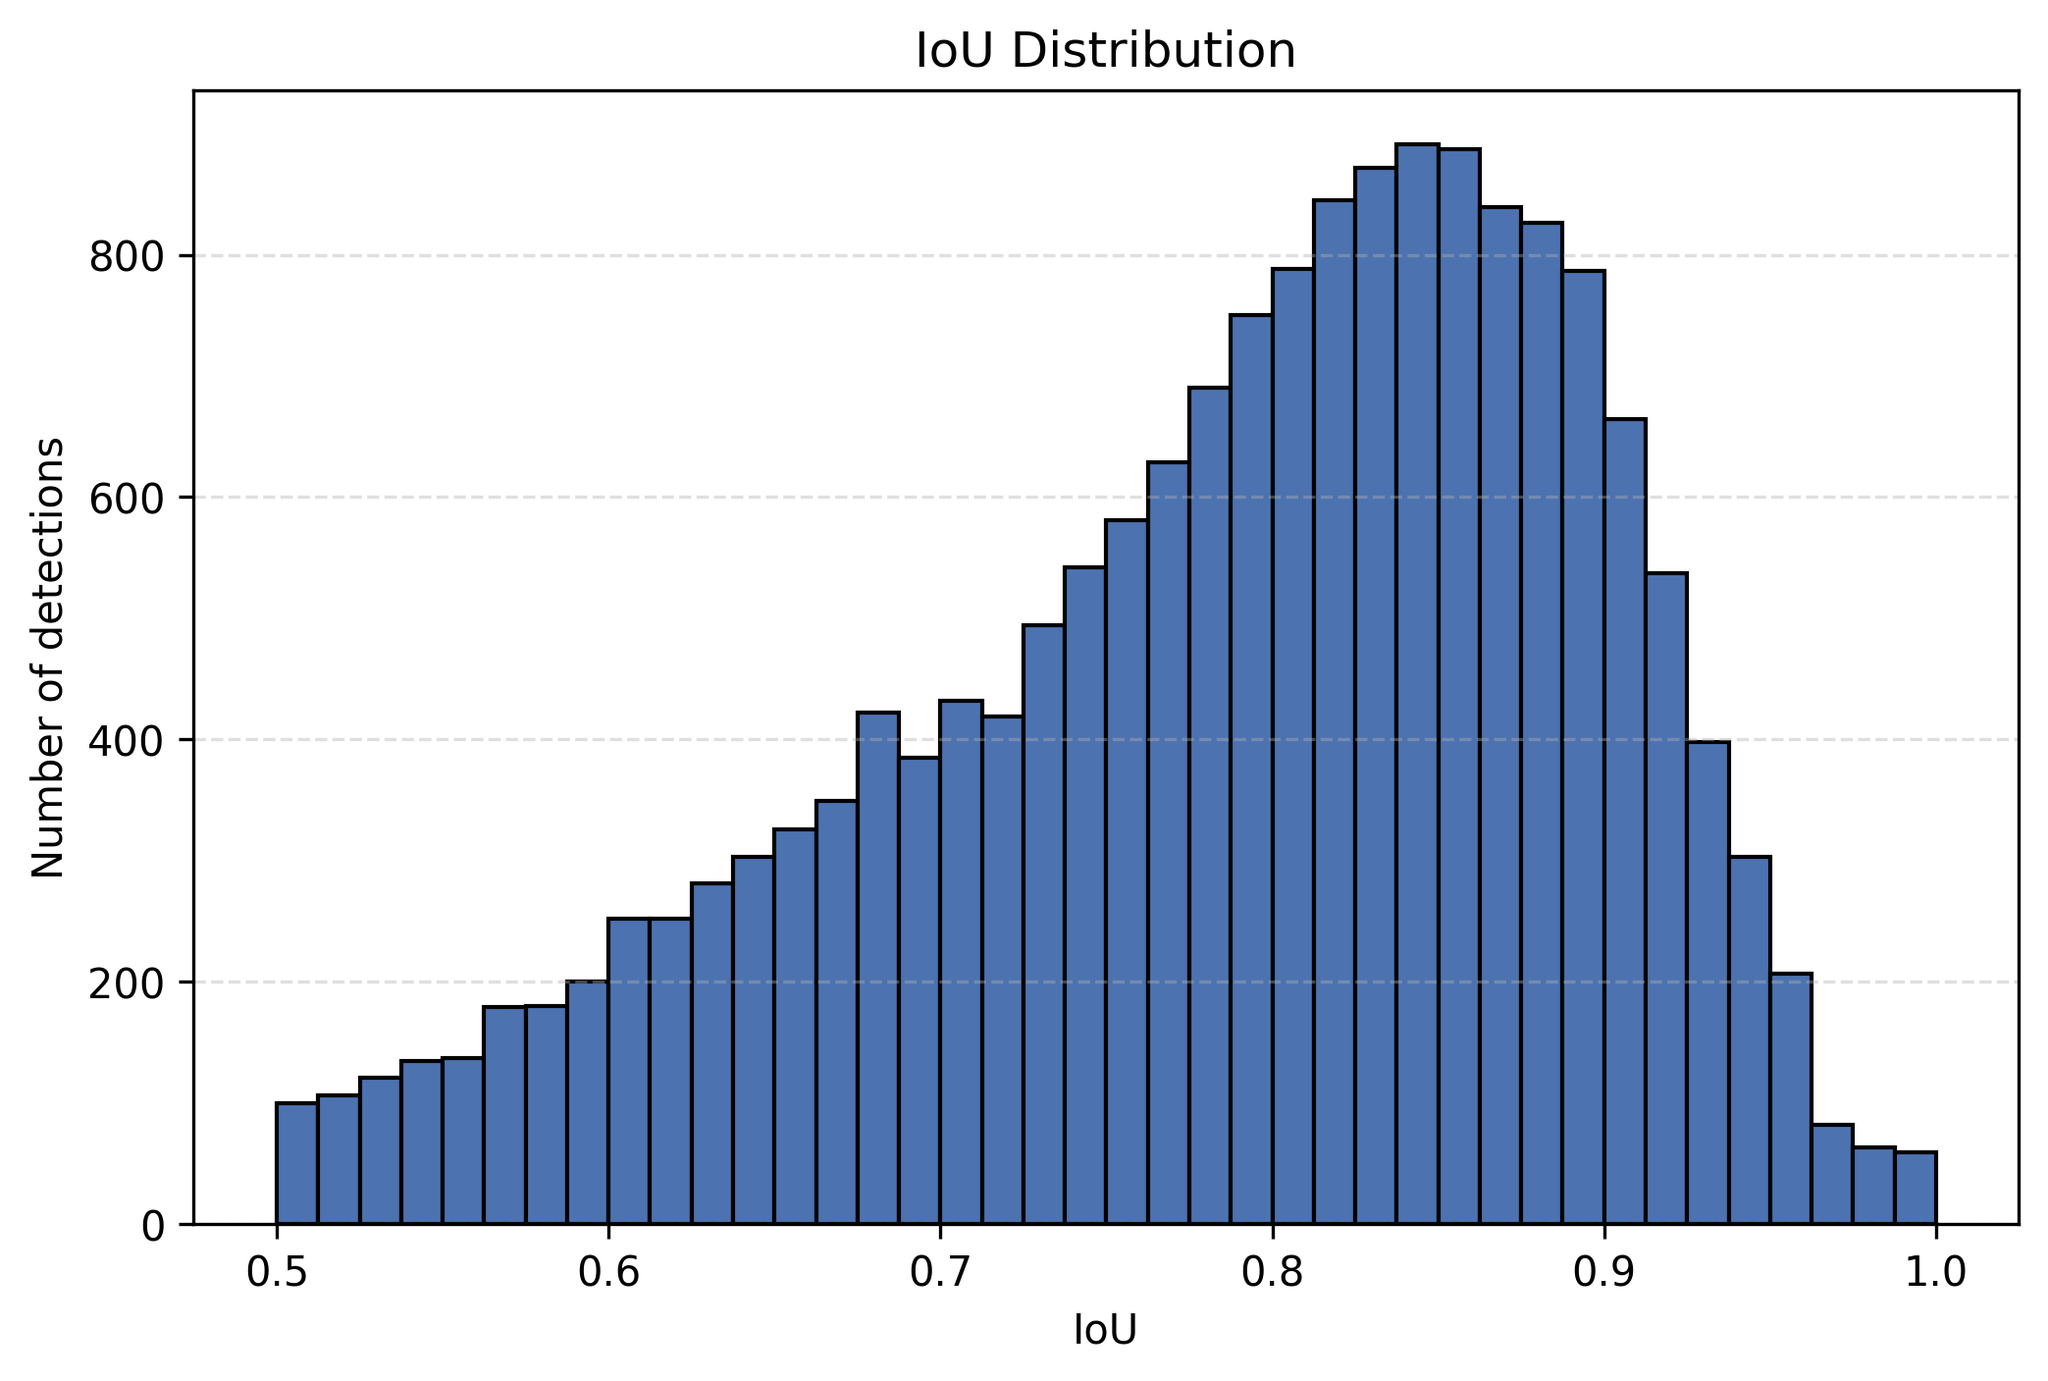
\includegraphics[width=0.6\textwidth]{images/iou_distribution.png}
  \caption{The IoU distribution.}
  \label{fig:iou}
\end{figure}

\noindent Most detections fall within the 0.75–0.90 IoU range, with the highest concentration around 0.85, indicating strong overlap between predicted and ground-truth text regions. Only a small portion of detections appear near the lower IoU threshold (0.50–0.65), which typically corresponds to slightly misaligned bounding boxes or partially detected text areas. Overall, these results indicate that the detection model provides accurate and reliable text localization for receipt images.
\vspace{0.5cm}

\noindent The text recognition performance is evaluated using Character Error Rate (CER), Word Error Rate (WER), and Line Accuracy.
\vspace{0.5cm}

\noindent The model achieves a CER of 12.04\%, corresponding to a character-level accuracy of 87.96\%. The WER reaches 64.89\%, while the line accuracy is 63.99\%, meaning that approximately 64\% of text lines are recognized perfectly.

\begin{figure}[H]
  \centering
  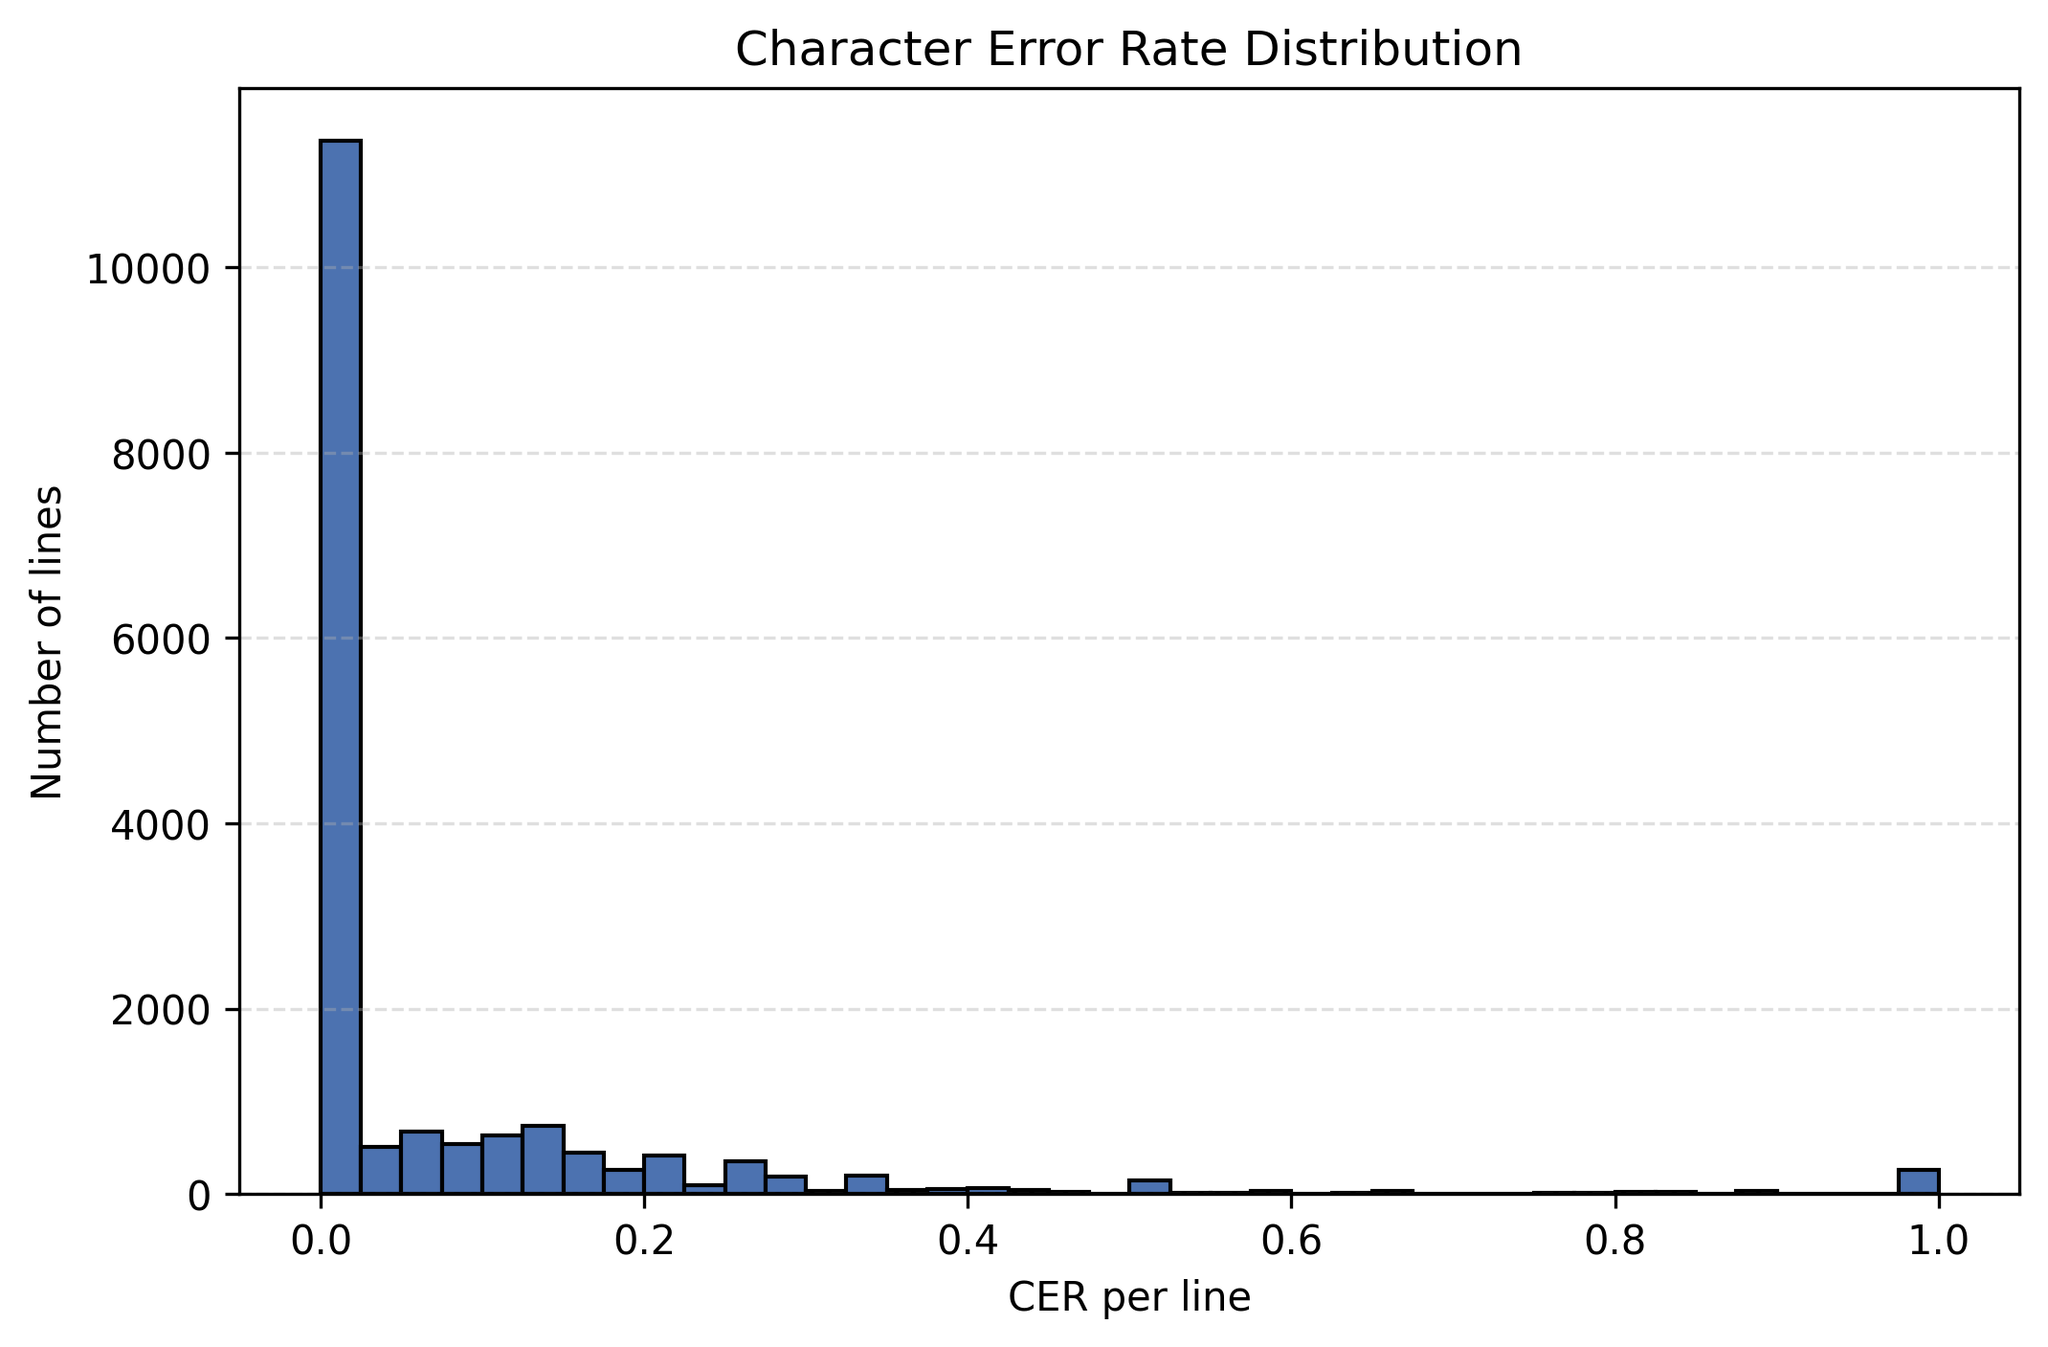
\includegraphics[width=0.6\textwidth]{images/cer_distribution.png}
  \caption{The CER distribution.}
\end{figure}

\noindent The distribution indicates that a large proportion of text lines have CER values close to zero, suggesting that the predicted text matches the ground truth for many instances. However, a smaller number of lines exhibit higher error rates due to recognition challenges in certain cases.

\begin{figure}[H]
  \centering
  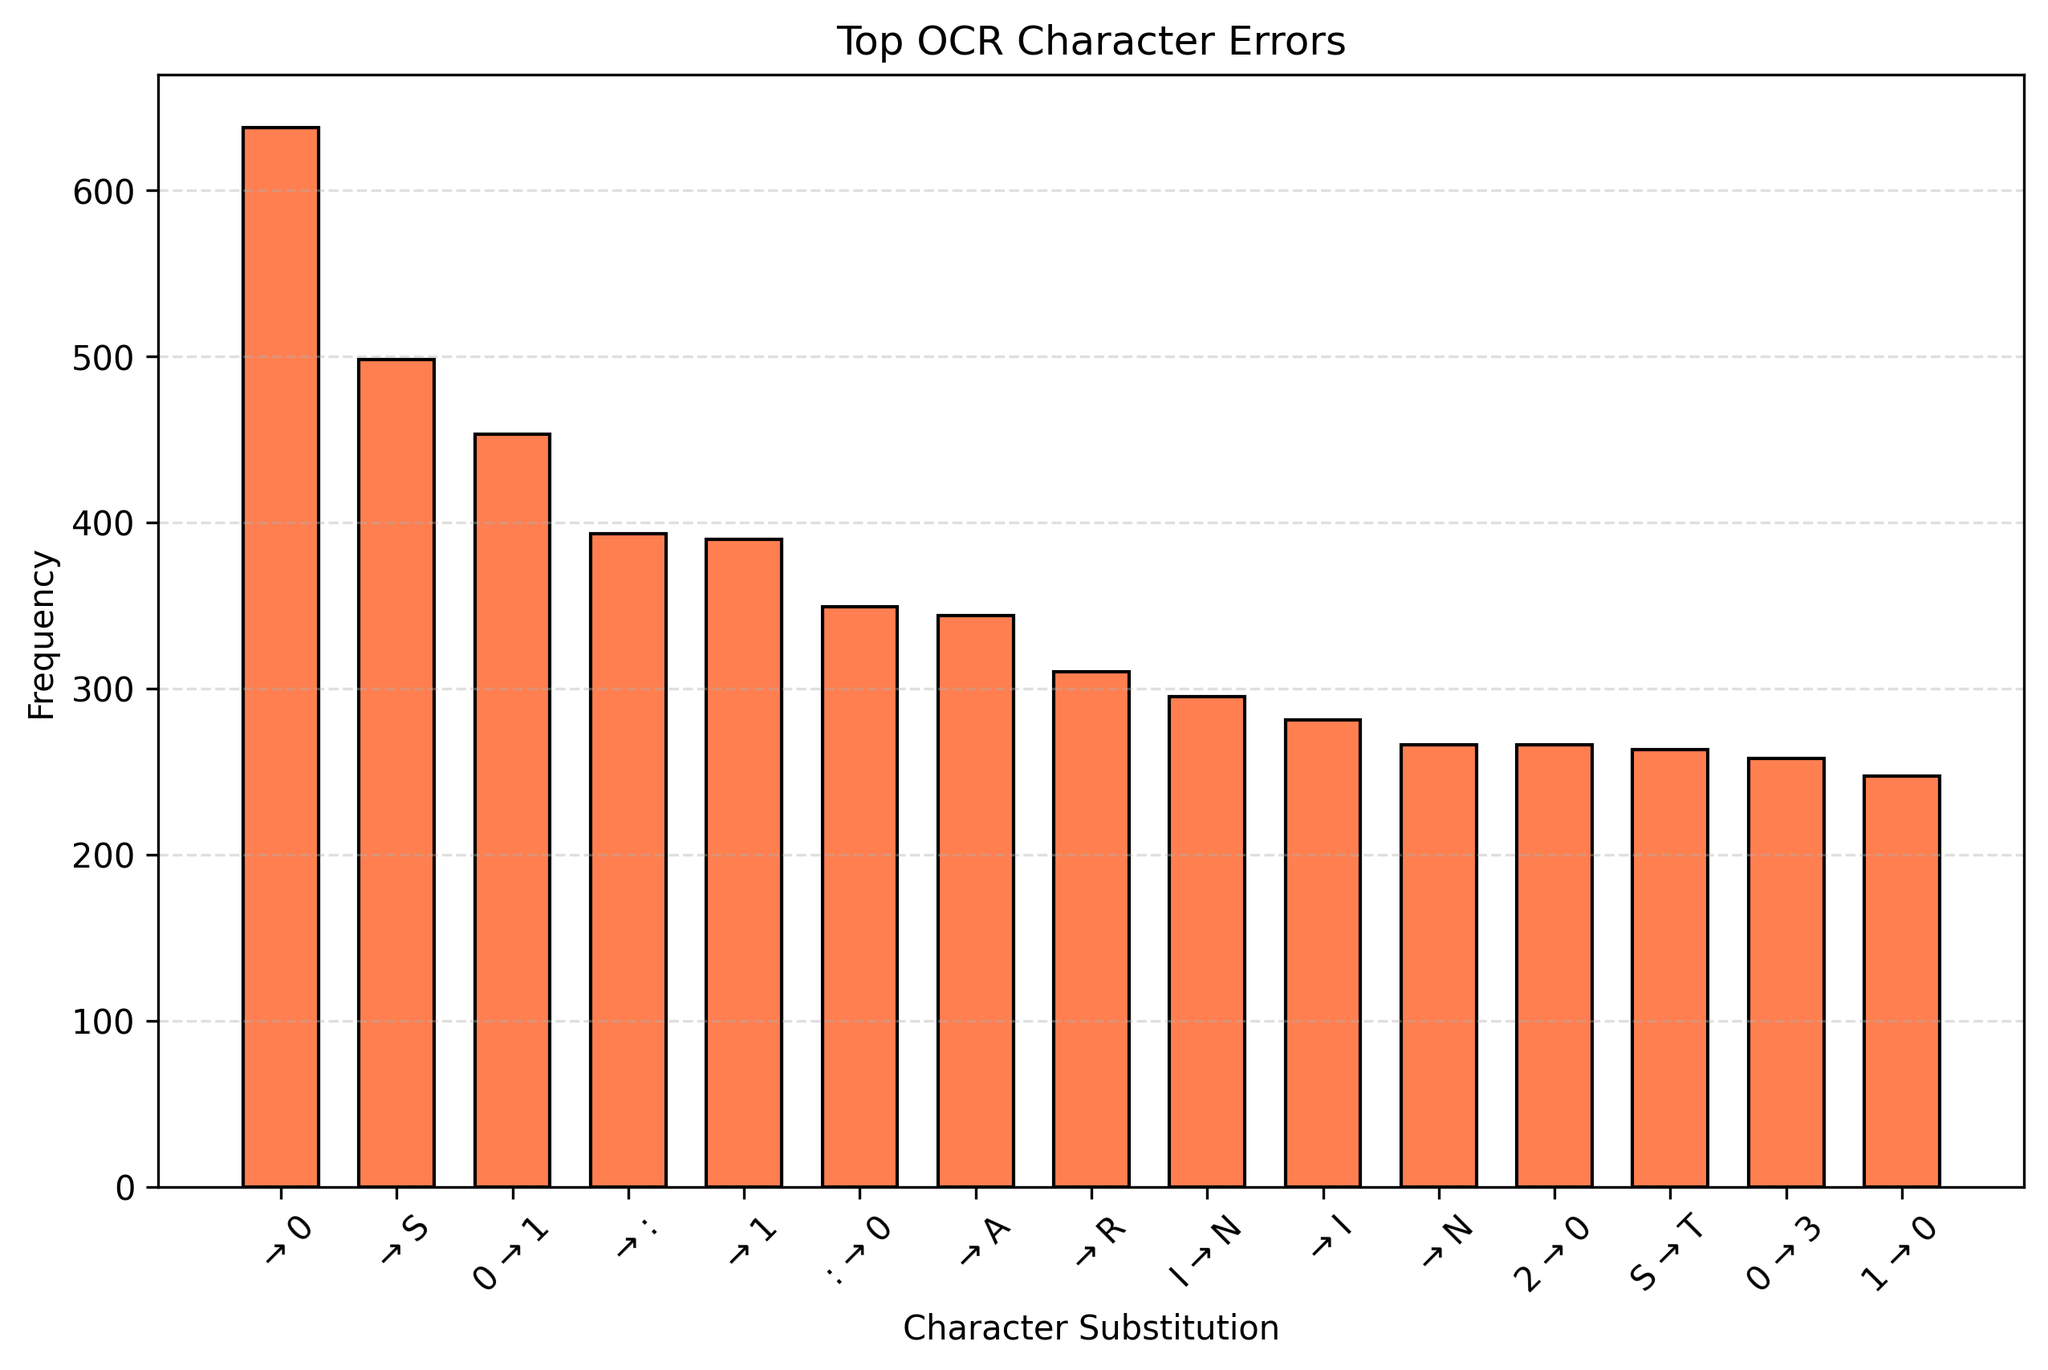
\includegraphics[width=0.6\textwidth]{images/top_ocr_errors.png}
  \caption{The most frequent character substitution errors.}
  \label{fig:iou}
\end{figure}

\noindent An analysis of character-level errors reveals common confusions between visually similar characters. The most frequent substitutions include “O → 0”, “S → 5”, and “0 → 1”, along with punctuation-related errors. These mistakes are typical in receipt OCR because many characters share similar visual structures and appear in small printed fonts.
\vspace{0.5cm}

\noindent Overall, the recognition model achieves high character-level accuracy, while most remaining errors are associated with visually ambiguous characters or challenging image conditions in receipt images.



\subsection{Example Output}